% A LaTeX template for EXECUTIVE SUMMARY of the MSc Thesis submissions to 
% Politecnico di Milano (PoliMi) - School of Industrial and Information Engineering
%
% P. F. Antonietti, S. Bonetti, A. Gruttadauria, G. Mescolini, A. Zingaro
% e-mail: template-tesi-ingind@polimi.it
%
% Last Revision: October 2021
%
% Copyright 2021 Politecnico di Milano, Italy. Inc. All rights reserved.

\documentclass[11pt,a4paper,twocolumn]{article}

%------------------------------------------------------------------------------
%	REQUIRED PACKAGES AND  CONFIGURATIONS
%------------------------------------------------------------------------------
% PACKAGES FOR TITLES
\usepackage{titlesec}
\usepackage{color}

% PACKAGES FOR LANGUAGE AND FONT
\usepackage[utf8]{inputenc}
\usepackage[english]{babel}
\usepackage[T1]{fontenc} % Font encoding

% PACKAGES FOR IMAGES
\usepackage{graphicx}
\graphicspath{{./Images/}{./Images/Template/}} % Path for images' folder
\usepackage{eso-pic} % For the background picture on the title page
\usepackage{subfig} % Numbered and caption subfigures using \subfloat
%\usepackage{caption} % Coloured captions
\usepackage{transparent}

% STANDARD MATH PACKAGES
\usepackage{amsmath}
\usepackage{amsthm}
\usepackage{bm}
\usepackage[overload]{empheq}  % For braced-style systems of equations

% PACKAGES FOR TABLES
\usepackage{tabularx}
\usepackage{longtable} % tables that can span several pages
\usepackage{colortbl}

% PACKAGES FOR ALGORITHMS (PSEUDO-CODE)
\usepackage{algorithm}
\usepackage{algorithmic}

% PACKAGES FOR REFERENCES & BIBLIOGRAPHY
\usepackage[colorlinks=true,linkcolor=black,anchorcolor=black,citecolor=black,filecolor=black,menucolor=black,runcolor=black,urlcolor=black]{hyperref} % Adds clickable links at references
%\usepackage{cleveref}
\usepackage[square, numbers, sort&compress]{natbib} % Square brackets, citing references with numbers, citations sorted by appearance in the text and compressed
\bibliographystyle{abbrvnat} % You may use a different style adapted to your field

% PACKAGES FOR THE APPENDIX
\usepackage{appendix}

% PACKAGES FOR ITEMIZE & ENUMERATES 
\usepackage{enumitem}

% OTHER PACKAGES
\usepackage{amsthm,thmtools,xcolor} % Coloured "Theorem"
\usepackage{comment} % Comment part of code
\usepackage{fancyhdr} % Fancy headers and footers
\usepackage{lipsum} % Insert dummy text
\usepackage{tcolorbox} % Create coloured boxes (e.g. the one for the key-words)
\usepackage{stfloats} % Correct position of the tables

%-------------------------------------------------------------------------
%	NEW COMMANDS DEFINED
%-------------------------------------------------------------------------
% EXAMPLES OF NEW COMMANDS -> here you see how to define new commands
\newcommand{\bea}{\begin{eqnarray}} % Shortcut for equation arrays
\newcommand{\eea}{\end{eqnarray}}
\newcommand{\e}[1]{\times 10^{#1}}  % Powers of 10 notation
\newcommand{\mathbbm}[1]{\text{\usefont{U}{bbm}{m}{n}#1}} % From mathbbm.sty
\newcommand{\pdev}[2]{\frac{\partial#1}{\partial#2}}
% NB: you can also override some existing commands with the keyword \renewcommand

%----------------------------------------------------------------------------
%	ADD YOUR PACKAGES (be careful of package interaction)
%----------------------------------------------------------------------------

\usepackage[threshold=1, thresholdtype=words]{csquotes}
\usepackage{booktabs}
\usepackage[capitalize]{cleveref}
\usepackage{dsfont}
\usepackage[skip=5pt]{caption}
\usepackage[export]{adjustbox}
\usepackage{makecell}
\usepackage{multirow}
\usepackage{hhline}
\usepackage{CJKutf8}
\usepackage{microtype}

% Do not change Configuration_files/config.tex file unless you really know what you are doing. 
% This file ends the configuration procedures (e.g. customizing commands, definition of new commands)
% Define blue color typical of polimi
\definecolor{bluepoli}{cmyk}{0.4,0.1,0,0.4}

% Custom theorem environments
\declaretheoremstyle[
  headfont=\color{bluepoli}\normalfont\bfseries,
  bodyfont=\color{black}\normalfont\itshape,
]{colored}

% Set-up caption colors
\captionsetup[figure]{labelfont={color=bluepoli}} % Set colour of the captions
\captionsetup[table]{labelfont={color=bluepoli}} % Set colour of the captions
\captionsetup[algorithm]{labelfont={color=bluepoli}} % Set colour of the captions

\theoremstyle{colored}
\newtheorem{theorem}{Theorem}[chapter]
\newtheorem{proposition}{Proposition}[chapter]

% Enhances the features of the standard "table" and "tabular" environments.
\newcommand\T{\rule{0pt}{2.6ex}}
\newcommand\B{\rule[-1.2ex]{0pt}{0pt}}

% Pseudo-code algorithm descriptions.
\newcounter{algsubstate}
\renewcommand{\thealgsubstate}{\alph{algsubstate}}
\newenvironment{algsubstates}
  {\setcounter{algsubstate}{0}%
   \renewcommand{\STATE}{%
     \stepcounter{algsubstate}%
     \Statex {\small\thealgsubstate:}\space}}
  {}

% New font size
\newcommand\numfontsize{\@setfontsize\Huge{200}{60}}

% Title format: chapter
\titleformat{\chapter}[hang]{
\fontsize{50}{20}\selectfont\bfseries\filright}{\textcolor{bluepoli} \thechapter\hsp\hspace{2mm}\textcolor{bluepoli}{|   }\hsp}{0pt}{\huge\bfseries \textcolor{bluepoli}
}

% Title format: section
\titleformat{\section}
{\color{bluepoli}\normalfont\LARGE\bfseries}
{\color{bluepoli}\thesection.}{1em}{}

% Title format: subsection
\titleformat{\subsection}
{\color{bluepoli}\normalfont\Large\bfseries}
{\color{bluepoli}\thesubsection.}{1em}{}

% Title format: subsubsection
\titleformat{\subsubsection}
{\color{bluepoli}\normalfont\large\bfseries}
{\color{bluepoli}\thesubsubsection.}{1em}{}

% Shortening for setting no horizontal-spacing
\newcommand{\hsp}{\hspace{0pt}}

\makeatletter
% Renewcommand: cleardoublepage including the background pic
\renewcommand*\cleardoublepage{%
  \clearpage\if@twoside\ifodd\c@page\else
  \null
  \AddToShipoutPicture*{\BackgroundPic}
  \thispagestyle{empty}%
  \newpage
  \if@twocolumn\hbox{}\newpage\fi\fi\fi}
\makeatother

%For correctly numbering algorithms
\numberwithin{algorithm}{chapter}


%----------------------------------------------------------------------------
%	ADD YOUR DEFINITIONS AND COMMANDS (be careful of existing commands)
%----------------------------------------------------------------------------

\newcommand{\gbm}[1]{\bm{\mathbf{#1}}} % General Bold Math for both greek and latin letters

\renewcommand\mkblockquote[4]{\leavevmode\llap{``}\textit{#1#2#3}''#4} % Blockquote quotation marks

%\setlength{\jot}{12pt} % Vertical equation spacing

\newcommand{\rowcolorhang}[1]{\rowcolor{#1}[\dimexpr\tabcolsep+0.1pt\relax]} % Add overang to table row coloring, to avoid vertical white lines

\interfootnotelinepenalty=1000000 % Avoid footnotes from breaking across pages
\captionsetup{belowskip=-6pt}

\creflabelformat{equation}{#2\textup{#1}#3} % Remove parentheses from cleveref equations

\renewcommand{\T}{\mathrm{T}} % Transpose

% Insert here the info that will be displayed into your Title page 
% -> title of your work
\renewcommand{\title}{Interpreting Large Language Models Through the Lens of \linebreak Embedding-Oriented Visualizations: Markov Models, Sankey \linebreak Diagrams and Comparative Approaches}
% -> author name and surname
\renewcommand{\author}{Davide Rigamonti}
% -> MSc course
\newcommand{\course}{Computer Science and Engineering - Ingegneria Informatica}
% -> advisor name and surname
\newcommand{\advisor}{Prof. Mark Carman}
% IF AND ONLY IF you need to modify the co-supervisors you also have to modify the file Configuration_files/title_page.tex (ONLY where it is marked)
\newcommand{\firstcoadvisor}{Nicolò Brunello} % insert if any otherwise comment
\newcommand{\secondcoadvisor}{Vincenzo Scotti} % insert if any otherwise comment
% -> academic year
\newcommand{\YEAR}{2024-2025}

%-------------------------------------------------------------------------
%	BEGIN OF YOUR DOCUMENT
%-------------------------------------------------------------------------
\begin{document}

%-----------------------------------------------------------------------------
% TITLE PAGE
%-----------------------------------------------------------------------------
% Do not change Configuration_files/TitlePage.tex (Modify it IF AND ONLY IF you need to add or delete the Co-advisors)
% This file creates the Title Page of the document
% DO NOT REMOVE SPACES BETWEEN LINES!

\twocolumn[{\begin{@twocolumnfalse}

\AddToShipoutPicture*{\BackgroundPic}

\hspace{-0.6cm}\includegraphics[width=0.6\textwidth]{logo_polimi_ing_indinf.pdf}

\vspace{-1mm}
\fontsize{0.3cm}{0.5cm}\selectfont \bfseries \textsc{\color{bluepoli} Executive Summary of the Thesis}\\

\vspace{-0.2cm}
\Large{\textbf{\color{bluepoli}{\title}}}\\

\vspace{-0.2cm}
\fontsize{0.3cm}{0.5cm}\selectfont \bfseries \textsc{\color{bluepoli} Laurea Magistrale in \course}\\

\vspace{-0.2cm}
\fontsize{0.3cm}{0.5cm} \selectfont \bfseries Author: \textsc{\textbf{\author}}\\

\vspace{-0.4cm}
\fontsize{0.3cm}{0.5cm}\selectfont \bfseries Advisor: \textsc{\textbf{\advisor}}\\

% if only ONE co-advisor is present:
%\vspace{-0.4cm}
%\fontsize{0.3cm}{0.5cm}\selectfont \bfseries Co-advisor: \textsc{\textbf{\firstcoadvisor}}\\
% if more than one co-advisors are present:
\vspace{-0.4cm}
\fontsize{0.3cm}{0.5cm}\selectfont \bfseries Co-advisors: \textsc{\textbf{\firstcoadvisor}}, \textsc{\textbf{\secondcoadvisor}}\\

\vspace{-0.4cm}
\fontsize{0.3cm}{0.5cm}\selectfont \bfseries Academic year: \textsc{\textbf{\YEAR}}

\small \normalfont

\vspace{11pt}

\centerline{\rule{1.0\textwidth}{0.4pt}}

\vspace{15pt}
\end{@twocolumnfalse}}]

\thispagestyle{plain} % In order to not show the header in the first page

%%%%%%%%%%%%%%%%%%%%%%%%%%%%%%
%%     THESIS MAIN TEXT     %%
%%%%%%%%%%%%%%%%%%%%%%%%%%%%%%

%-----------------------------------------------------------------------------
% INTRODUCTION
%-----------------------------------------------------------------------------
\section{Introduction}\label{sec:introduction}

With the growing popularity and pervasiveness of machine learning solutions applied to the realm of natural languages, \emph{interpretabilty} remains an increasingly relevant topic, still subject of extensive studies by experts in this field.
Interpretabilty in itself is far from being a novel concept, as from the early advent of machine learning there has always been the necessity of understanding the process by which an opaque model performs its inner computations.

Considering the introduction of the \emph{deep learning paradigm}, reducing human control over feature spaces, the need for interpretabilty spiked as models became more complex.
In particular, we are interested in a specific class of machine learning models that are currently considered state-of-the art in the Natural Language Processing (NLP): \emph{Large Language Models (or LLMs)}.

This work offers novel perspectives over the internal structure of LLMs through exploratory analyses, creation of tools, and experiments confirming and possibly improving existing hypotheses and observations in the interpretability field.
The overall approach is structured along three main research questions: 
\begin{itemize}[leftmargin=12pt]
    \item \textbf{``How can we visualize internal states of LLMs in an immediate and interactive Way?''} Focuses on developing an interactive visualization tool for LLMs, \emph{InTraVisTo (Inside Transformer Visualization Tool)}, designed to support machine learning researchers in hypothesis formulation by offering a unique perspective on the internal representations of LLMs.
    \item \textbf{``Do autoregressive LLMs retain linear properties in their embedding spaces?''} Assesses whether linearity properties persist in the embedding spaces of contemporary causal LLMs and whether they are consistent across various model architectures and sizes, highlighting differences between embedding and unembedding spaces.
    \item \textbf{``Is it Possible to Obtain First-order Predictions by Concatenating Embedding Spaces in LLMs?''} Explores whether the First Order Model (FOM), obtained by multiplying the embedding matrices of an LLM, can accurately represent a bigram Markov model over the original model's vocabulary.
\end{itemize}

%-----------------------------------------------------------------------------
% RELATED WORKS
%-----------------------------------------------------------------------------
\section{Related Works}\label{sec:related_works}
The field of Transformer interpretability has garnered significant attention over the past decade, resulting in a growing body of literature.
This section briefly reviews contributions and developments in this area, highlighting the foundational studies and recent advancements relevant to our research.
Specifically, we explore the foundation of \textbf{Mechanistic Interpretability (MI)}, which forms the basis of our work, and examine the concept of \textbf{linear representation hypothesis} along with its related works, which play a central role in our investigations.
In addition, we discuss elements of \textbf{vocabulary space decoding} and current state-of-the-art visualizations based on this technique.

\subsection{Mechanistic Interpretability}

\textbf{Mechanistic interpretability} offers a novel perspective over the NLP interpretability research field, its primary aim being the \emph{reverse-engineering} of language models (LMs) from an in-depth perspective~\cite{olah2022}.
Mechanistic interpretability was initially mentioned as being the main driving ideology behind the ``Transformer circuits thread''.
Nonetheless, the concept of MI is not limited to the application of circuits; envisioning MI as being characterized by a general bottom-up approach for interpreting LMs, allows its scope to extend to include earlier techniques such as the logit lens~\cite{nostalgebraist2020} and other probing methods.

\subsection{Linear Representation \texorpdfstring{ \\ }{} Hypothesis}

The \textbf{linear representation hypothesis}~\cite{park2023} posits that high-level concepts are represented linearly within the representation space of a language model.
The central idea for this hypothesis builds upon early findings of linearity inside the embedding space by~\citet{mikolov2013}, leading to the resolution of analogies and the presence of geometric properties as the direct consequences of a linear embedding space.

Another important aspect of the linear representation hypothesis is the presence of \emph{polysemanticity} and \emph{superposition} in the identified features spaces obtained via dimensionality reduction algorithms, resulting in distributed representations via information compression.
Many extend these observations to actual experiments, successfully proving the existence of superposition in simplified scenarios~\cite{elhage2022}.

\subsection{Vocabulary Space Decoding}

One of the most direct methods to comprehend a model's hidden representations is by employing its own vocabulary to derive plausible interpretations.
\textbf{Vocabulary space decoding} techniques are founded on this principle, by utilizing the model's existing vocabulary they can generate outputs that are immediately understandable and may unveil hidden patterns inside the model's generation process.

The first real implementation of vocabulary space decoding is \emph{logit lens}~\cite{nostalgebraist2020}, which proposed the decoding of interlayer hidden representation using the model's own unembedding matrix.
The contribution of logit lens was groundbreaking and, despite some acknowledged shortcomings by the author, inspired numerous similar techniques aimed at improving its design or offering alternative functionalities.

A more recent iteration of the vocabulary space decoding approach is the \emph{LM Transparency Tool (LM-TT)}~\cite{tufanov2024}, which is an exceptional toolkit offering interactive tools for analyzing the internal workings of Transformer models.
LM-TT builds on top of the circuital interpretation of the Transformer to visualize the information flow.
The LM-TT tool focuses on the visualization of the most relevant attention paths leading to the production of an embedding in the internal states of the Transformer.
Additionally, it also provides useful decoding information that can aid the interpretation of intermediate representations at varying degrees of granularity.

%-----------------------------------------------------------------------------
% INTRAVISTO
%-----------------------------------------------------------------------------
\section{InTraVisTo}\label{sec:intravisto}

We develop \emph{InTraVisTo}\footnote{\rlap{\url{https://github.com/daviderigamonti/InTraVisTo}}} as a tool designed to visualize internal states and the information flow within Transformer-based neural networks underlying modern LLMs.
It offers a wide array of functionalities and visualizations to NLP practitioners, which they can utilize to understand internal reasoning steps carried out by LLMs and, possibly, track down the causes of generation errors such as hallucinations.
As an interactive framework, InTraVisTo is able to modify and manipulate internal representations in order to enable small-scale causal investigations.
Moreover, InTraVisTo's implementation supports concurrent use by multiple users with the simultaneous loading of distinct LLMs at the same time, making it a flexible application capable of being deployed in a reproducible way for NLP researchers and practitioners.

This section explores the principal elements that comprise InTraVisTo, illustrating their design and explaining how they integrate their functionalities into the overall framework.
It is possible to identify three main components: the \textbf{decoding interface}, the \textbf{flow interface} and the \textbf{injection interface}.

\subsection{Decoding Interface}\label{ssec:intravisto_1}

Decoding the meaning of hidden state vectors at various depths of a Transformer stack is essential for providing an intuition as to how the model is working.
InTraVisTo allows decoding and inspection of the \emph{main four vectors} that compose each layer, while offering a human-interpretable representation of each hidden state by performing a decoding operation.
The four vectors correspond respectively to the output of the attention component, the intermediate state given by the addition of the attention component to the residual stream, the output of the feed-forward network component, and the layer output.
On the other hand, the decoding operation is carried out using a specialized decoder which, given a hidden state as input, finds related tokens from the model's vocabulary with the goal of returning an interpretable output as formalized in~\cref{eq:method_intravisto_decoding}.

\vspace{-12pt}
{
\medmuskip=0mu
\thinmuskip=1mu
\thickmuskip=0mu
\scriptspace=0pt
\begin{equation}
\label{eq:method_intravisto_decoding}
\hspace{-10pt}
\begin{aligned}
P(\,\cdot\,\mid \gbm{x}, d_\textit{\scalebox{.8}{dec}}, n_\textit{\scalebox{.8}{norm}}) \,&=\, P(\,\cdot\,\mid \gbm{x}, \gbm{W}_{d_\textit{\scalebox{.8}{dec}}}, N_{n_\textit{\scalebox{.8}{norm}}}) \\
&=\,\operatorname{softmax}\Bigl(N_{n_\textit{\scalebox{.8}{norm}}}(\gbm{x}) \cdot \gbm{W}_{d_\textit{\scalebox{.8}{dec}}}\Bigr)
\end{aligned}
\end{equation}
}%
\noindent Where $\gbm{W}_{d_\textit{dec}}$ represents the matrix of decoder weights according to the user decoder choice $d_\textit{dec}$, and $N_{n_\textit{norm}}$ is used to identify the normalization operation selected by the user through $n_\textit{norm}$.

Two natural choices for decoders are the transpose of the \emph{input embedding matrix} $\gbm{W}_\textit{in}^\T$ which the model uses to convert tokens into vectors at the input stage, and the \emph{output unembedding matrix} $\gbm{W}_\textit{out}$, which is used within the language modeling head to generate token outputs from internal vectors.
InTraVisTo also offers the possibility of decoding hidden states by \emph{interpolating} the input and output decoders based on the depth $\ell\in\{0,\ldots,L\}$ of the model layer to be decoded, we obtain a ``hybrid'' decoding weight matrix that acts as an equilibrium point calibrated on the current depth of the model.

\begin{figure}[tbh!]
    \centering
    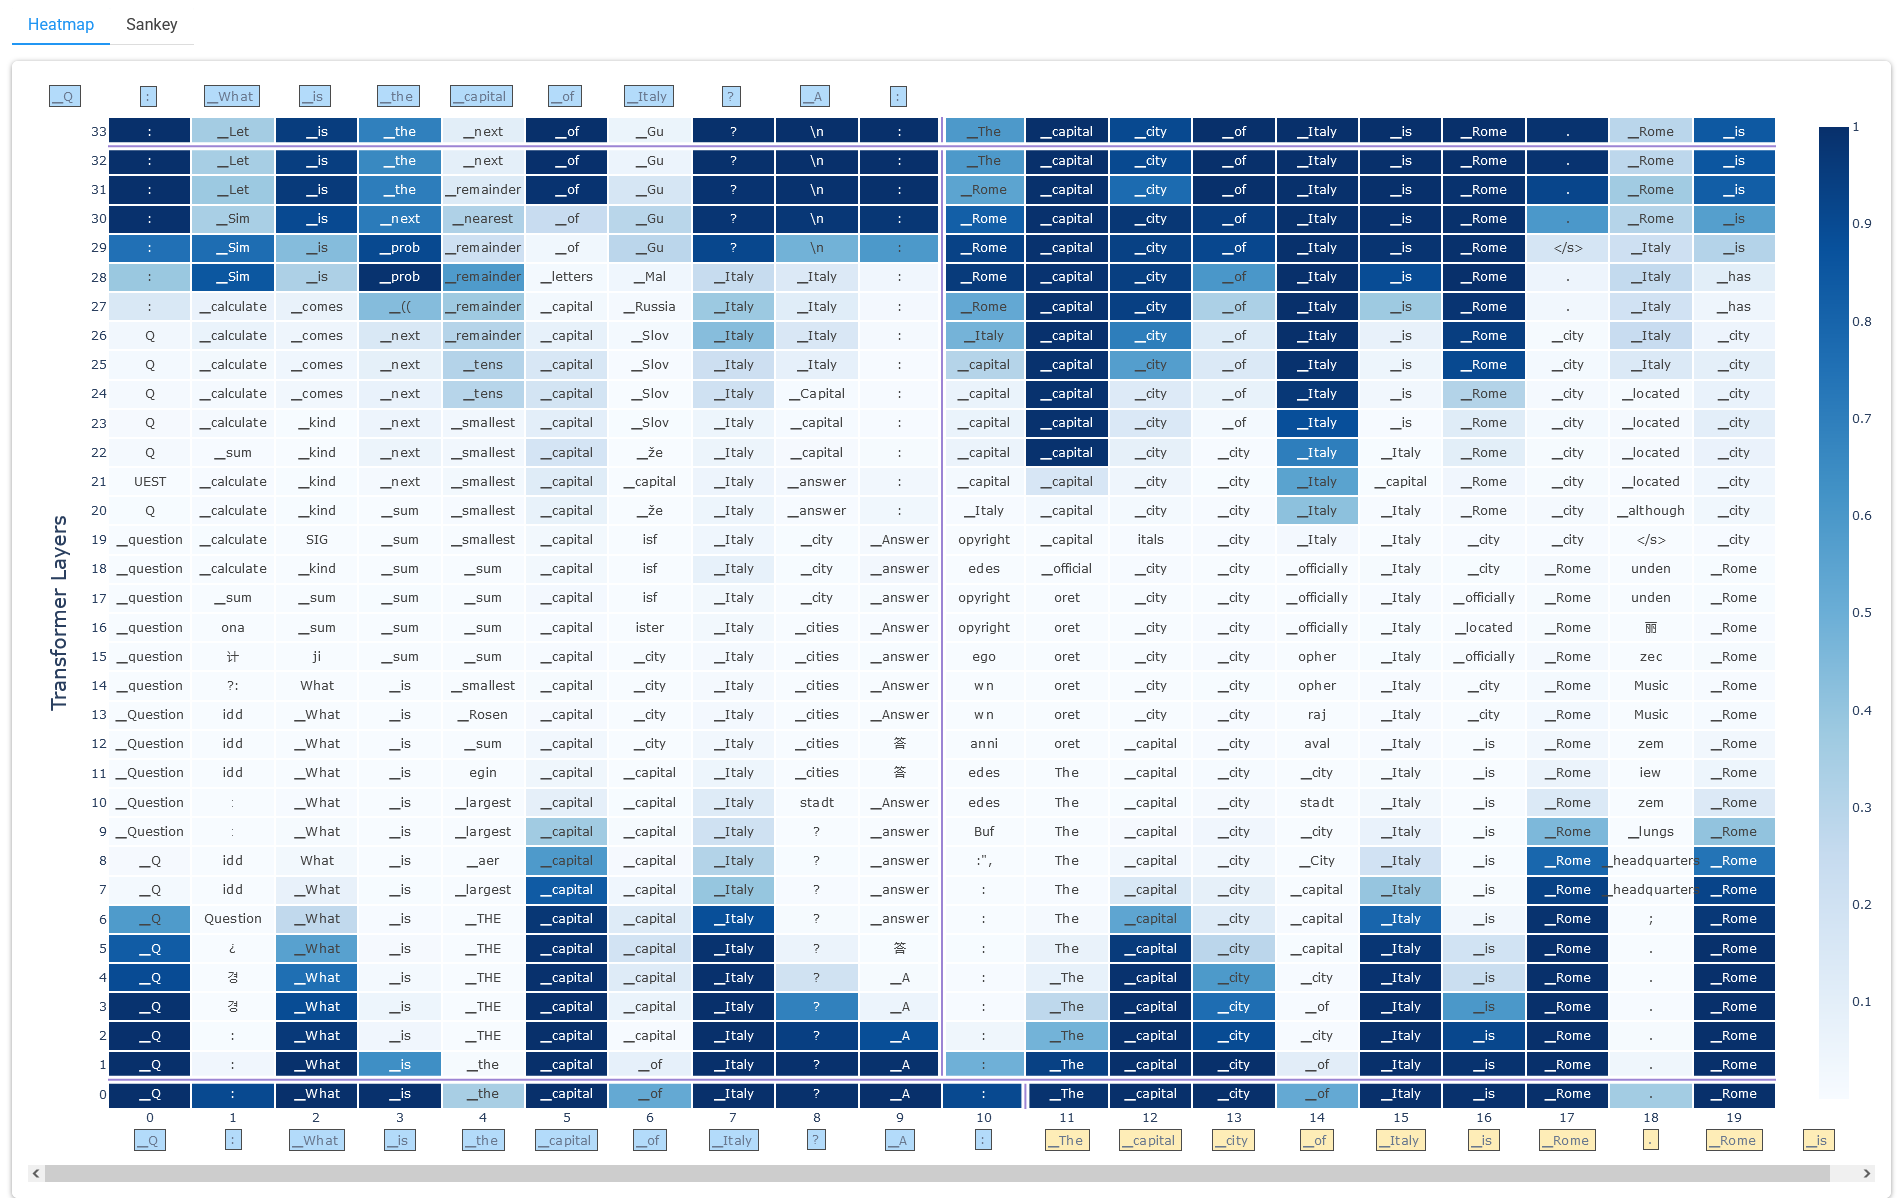
\includegraphics[width=0.47\textwidth]{exp_intravisto_1A_heatmap.png}
    \caption{InTraVisTo's heatmap visualization given the prompt \emph{``What is the capital of Italy?''} to Mistral, utilizing linear interpolation for decoding.}
    \label{fig:exp_intravisto_1_A}
\end{figure}

In~\cref{fig:exp_intravisto_1_A} we show InTraVisTo first visual output, obtained from a layer-by-layer model interpretation.Layers are stacked vertically, from the embedding layer at the bottom to the normalized outputs at the top, forming a grid where the x-axis represents token positions in the sequence and the y-axis represents layer numbers, resulting in a heatmap where each cell represents a token-layer combination containing the main decoded hidden state in token form.
By hovering on a cell, a pop-up with other possible decoded tokens (secondary representation) along with additional information appears.

The generation of the heatmap requires the user to choose a \emph{target embedding}, a \emph{decoding strategy} and a \emph{probability} to display.
The embedding refers to the position of the hidden state vector to be decoded within the layer.
Conversely, the decoding strategy choice refers to the decoding matrix employed during the decoding process of each visualized hidden state.
Finally, the probability selector directly affects the quantity used to weight the color grading in the heatmap, and is normally tied to the probability of the obtained decoding for each cell as formalized in~\cref{eq:method_intravisto_decoding}.

\subsection{Flow Interface}

The second visualization provided by InTraVisTo is a \emph{Sankey diagram} that aims to depict the information flow through the Transformer network (\cref{fig:exp_intravisto_2_A}).

\begin{figure}[tbh!]
    \centering
    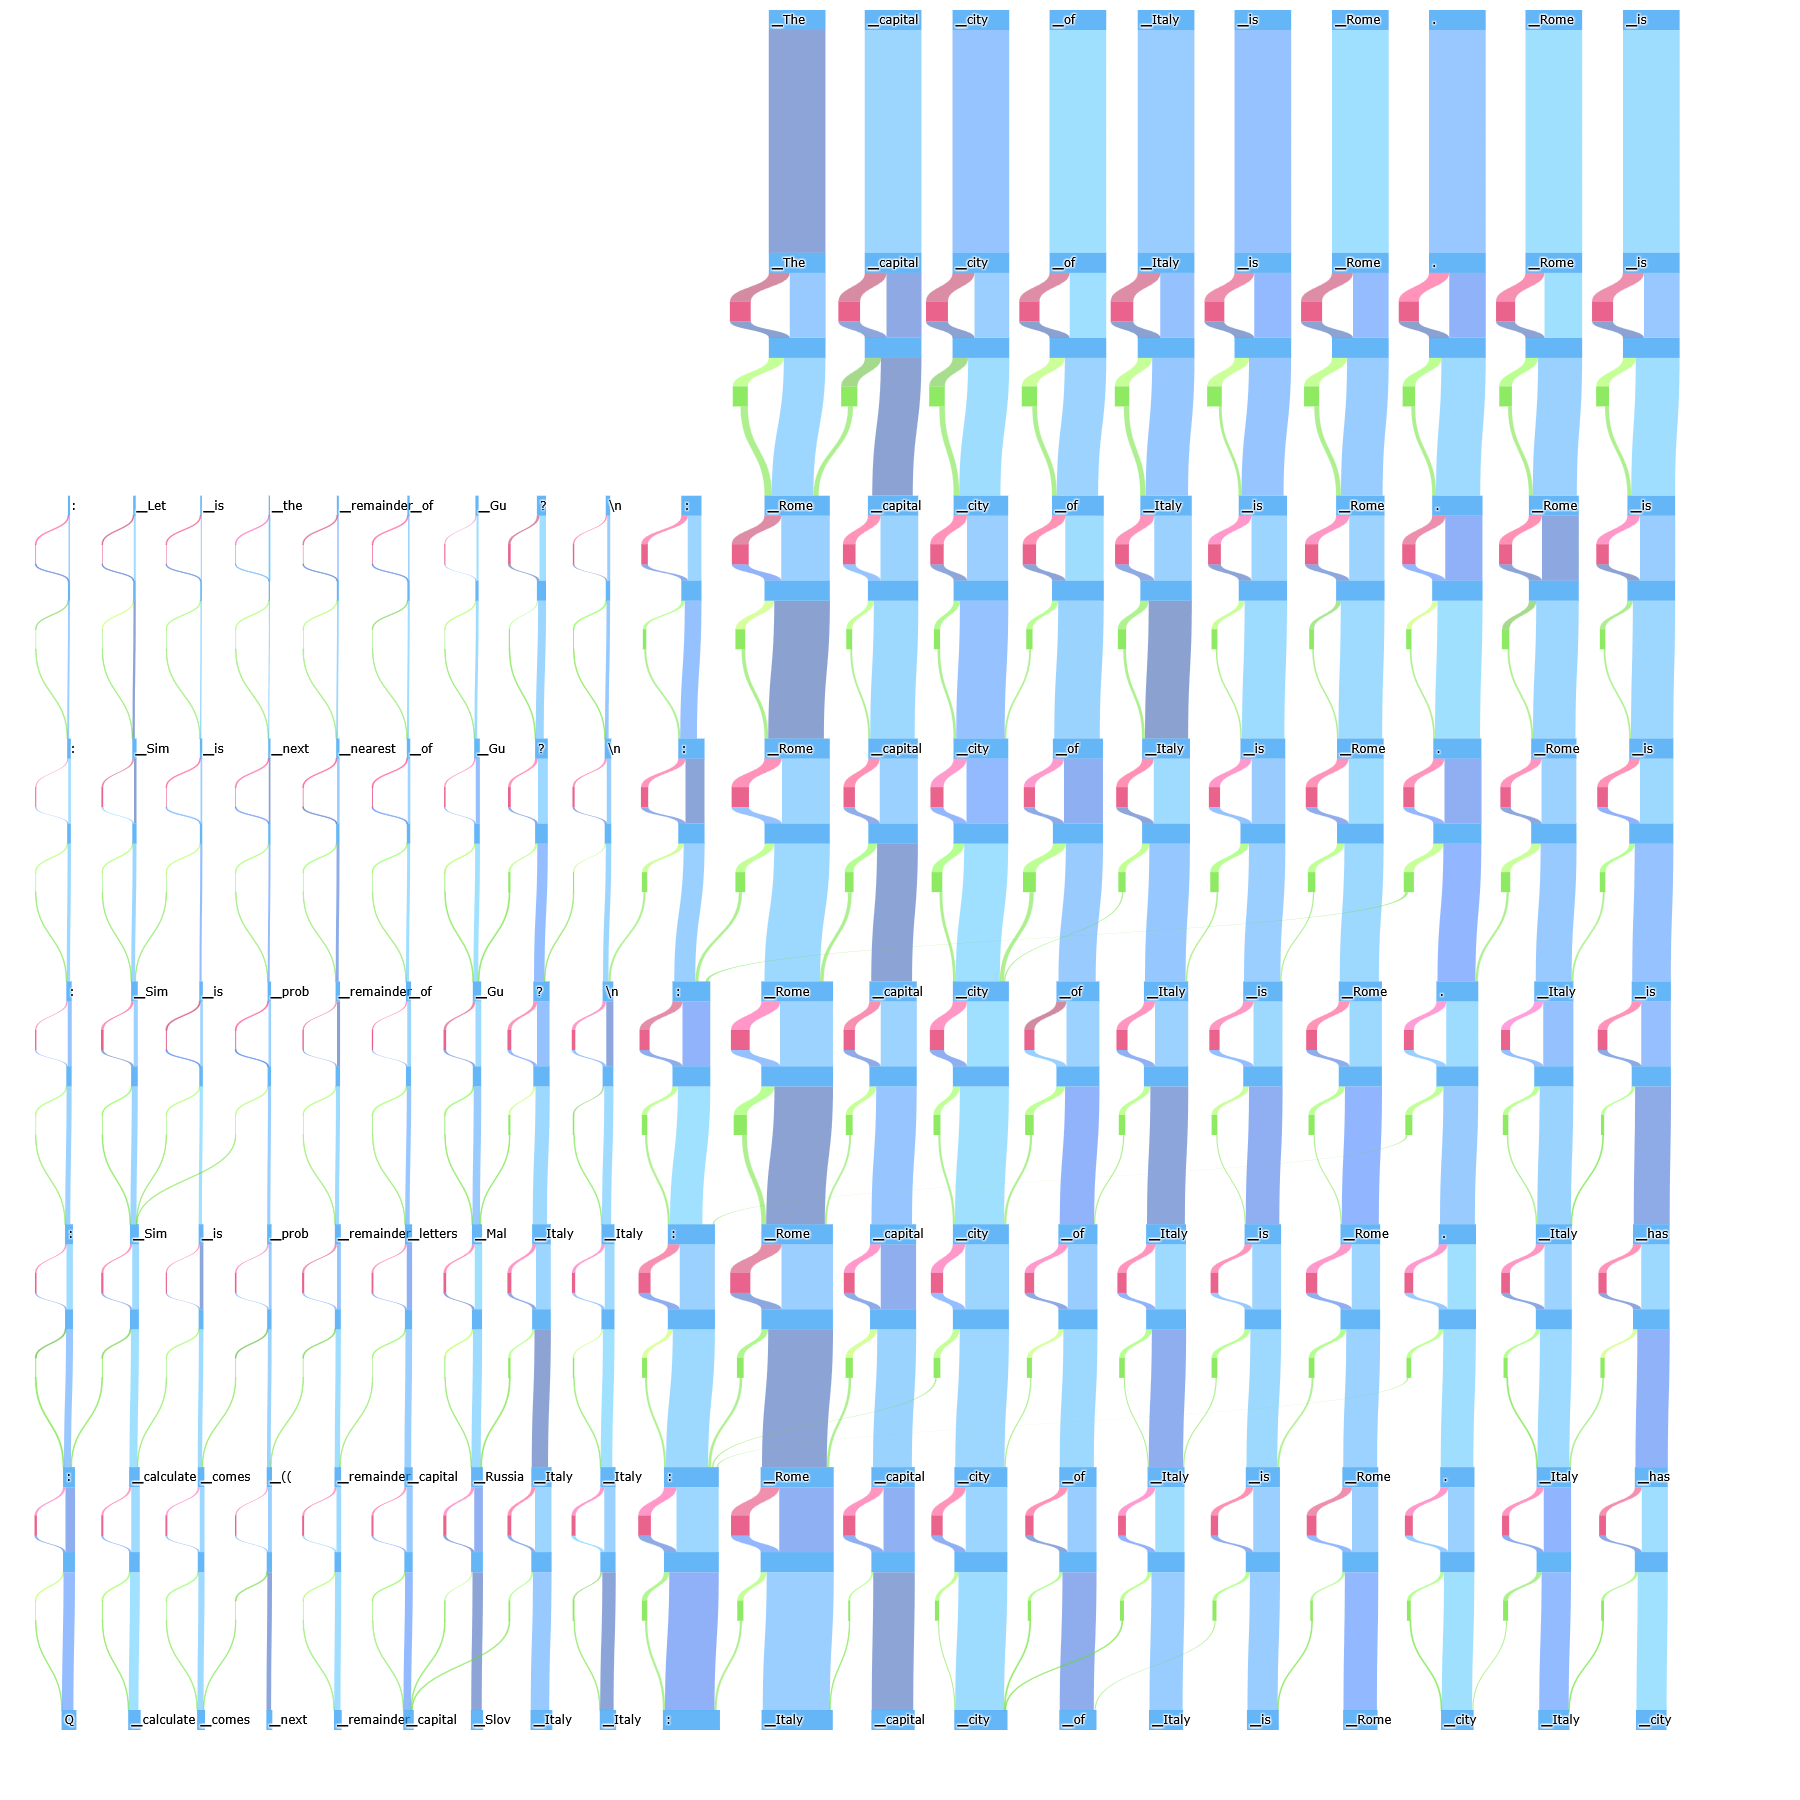
\includegraphics[width=0.45\textwidth]{exp_intravisto_2A_sankey.png}
    \caption{InTraVisTo's Sankey diagram visualization of the last 7 layers given the prompt \emph{``What is the capital of Italy?''} to Mistral.}
    \label{fig:exp_intravisto_2_A}
    \vspace{-10pt}
\end{figure}

Nodes in the diagram depict all hidden states contained in each layer, visualizing the four vectors referenced in~\cref{ssec:intravisto_1} at the same time.
Like in the heatmap, nodes display the main decoding result as their label and, when hovered upon, show additional information in the form of a pop-up tooltip containing secondary representations.
Output nodes' tooltips also include the \emph{decoded difference from the previous layer}, obtained between the current and previous output states with the goal of trying to visualize in a human interpretable way the information added by the current layer relative to the previous one.

On the other hand, edges represent the amount of relevance carried by the residual stream, showing how components accumulate or disperse this flow as they process information scattered across the model.
The flow originates from the topmost layer of nodes, equally split between them, and is recursively computed considering the contributions of each encountered node in a way that no amount of flow is ever lost between layers.
If the user inspects a specific cell in the heatmap by clicking on it, the Sankey diagram adapts by recalculating the flow considering the clicked node as the sole topmost node, consequently accounting for $100\%$ of the flow.
Nodes are subdivided into three color-coded categories for convenience: \emph{intermediate and output nodes} in blue, \emph{attention nodes} in green and \emph{feed-forward nodes} in pink.
Moreover, flows exiting from each node inherit the color of their originating node and are given a further shading factor that is proportional to the \emph{Kullback-Leibler divergence} between the decoded hidden state distributions of the nodes that they connect.
This allows users to appreciate in an immediate way states that exhibit rapid changes in distribution, thus providing a better localization for possible zones of interest.

\subsection{Injection Interface}

InTraVisTo is designed as an interactive tool, and \emph{embedding injection} is another feature to enhance understanding of the of Transformers internals.
Injections substitute hidden states with custom embedding representations, forcing the model to adjust its behavior based on the injected information.
They are performed by clicking on a cell in the heatmap; this action opens a pop-up menu prompting the user for a string of text with the purpose of being encoded into an embedding representation and injected inside the selected hidden state, the injection technique specifying how the new embedding is integrated into the preexisting state, the position of the injection inside the selected layer, the decoding technique used to interpret the aforementioned string of text, and for the option to normalize the injected embedding.
Once a valid injection is compiled and added, a small card summarizing the injection appears at the top of the interface.

Injections can also be performed in the Sankey diagram by clicking on any visible node, triggering the same pop-up menu described above.
If the chosen node corresponds to a feed-forward or an attention node, there is an additional option that allows the user to remove the node, performing an \emph{ablation}.
Ablations are processed similarly to injections and remove the selected node by nullifying its contribution to the residual, so its hidden state is still decoded and visible from the heatmap but does not influence the rest of the model.

%-----------------------------------------------------------------------------
% EXPERIMENTS
%-----------------------------------------------------------------------------
\section{Experiments}\label{sec:experiments}

Besides the primary task of developing of InTraVisTo, as examined in~\cref{sec:intravisto}, we also propose two separate experiments in order to address the remaining research questions.
These experiments take the form of an in-depth analysis on embeddings through word analogies for the second research question, and an exploration of first order predictions for the last research question.
Moreover, the main body of work includes a case study that exemplifies the usage of InTraVisTo for the first research question.

\subsection{Embedding Analysis}

In this experiment we establish whether geometric relationships can still be modeled inside the input or output embedding space of recent LLM architectures by direct experimentation on \emph{word analogy tasks}, as originally illustrated in~\citet{mikolov2013}.
Solving word analogies showcases an embedding space's ability to model word semantics in a relatively consistent way, implying the existence of embedding dimensions with associated meanings (even if overlapping or under superposition, as noted by~\citet{elhage2022}).

As a starting point, we directly compare the performance of the input embeddings belonging to various state-of-the art and older models over the defined analogy task.
We also take into consideration the unembedding layer of models, which shares a common structure with the actual embedding matrix and should provide meaningful experimental results.
Additionally, inspired by the decoding approach introduced for InTraVisTo, we also perform analogy experiments on interpolated embeddings.

We run these experiments utilizing GPT-2, Mistral 7B v0.3, Llama 2 7B, Llama 3 8B, Phi 3.5 mini instruct, Gemma 2 2B, GloVe, word2vec and BERT large uncased.
The dataset includes both the original Google analogy dataset~\cite{mikolov2013} and the Bigger Analogy Test Set (BATS)~\cite{drozd2016}, used either in complete form or by filtering out analogies that cannot be encoded using single tokens from the models' vocabularies.

\begin{figure}[tbh!]
    \vspace{-10pt}
    \centering
    \subfloat[\label{fig:exp_emb_1_A1}]{%
        \includegraphics[width=0.22\textwidth]{exp_emb_1A_topk_l2-m-l3.pdf}%
    }%
    \subfloat[\label{fig:exp_emb_1_A2}]{%
        \includegraphics[width=0.22\textwidth]{exp_emb_1A_topk_g2-p3-b.pdf}%
    }%
    \quad%
    \subfloat[\label{fig:exp_emb_1_A3}]{%
        \includegraphics[width=0.22\textwidth]{exp_emb_1A_topk_w2v-gv.pdf}%
    }%
    \subfloat[\label{fig:exp_emb_1_A4}]{%
        \includegraphics[width=0.22\textwidth]{exp_emb_2B_topk_m-7-15-8-io.pdf}%
    }%
    \caption{Top-$k$ accuracy on the word analogies task for various models.}
    \label{fig:exp_emb_1_A}
    \vspace{-5pt}
\end{figure}

From the obtained results we can affirm that LLMs are able to retain a surprising amount of semantic relationships inside their embeddings, despite the fact that \emph{sub-word tokenization} actively works against the accumulation of meaning for token representations.
Their performance on the selected tasks is comparable, if not greater than less recent models used as baselines, as shown in~\cref{fig:exp_emb_1_A1,fig:exp_emb_1_A2,fig:exp_emb_1_A3}.
However, from~\cref{fig:exp_emb_1_A1,fig:exp_emb_1_A2}, we can observe that very large, recent models such as Llama 3 and Gemma may be trending towards a direction of semantic impoverishment of the embedding space, whereas slightly older LLMs like Llama 2 and Mistral, as well as models designed for compactness and portability, such as Phi 3.5, still preserve many of the original embedding space properties.

From~\cref{fig:exp_emb_1_A4}, we can conclude that input embeddings are generally better suited for resolving analogies and, by extension, inherently contain a greater amount of semantic information with respect to output embeddings, and in addition, interpolated embedding spaces retain at least the same amount of information as the original embeddings.

\subsection{First Order Prediction}

A \emph{First Order Model (FOM)} is derived by removing all intermediate architectural components from an LLM, retaining only the input and output embedding layers along with the residual connections joining them.
This transformation can be seen as the creation of a \emph{Markov model} whose transition matrix is given by the product of the input and output embedding matrices.
Although past work has theorized that FOMs represent Markov models on a small scale~\cite{elhage2021}, in this experiment, we investigate if FOMs derived from actual LLMs exhibit varying degrees of Markovian behavior, while also considering the possibility of FOM transition matrices approximating identity matrices, effectively modeling \emph{weight tying}.

We introduce various approaches to explore the main inquiry: we start by performing a \emph{naïve direct comparison} between transition matrices, followed by the use of \emph{set similarity metrics} (such as top-$k$ accuracy, Jaccard similarity and overlap coefficient) to obtain more reliable estimates, and ending with the computation of \emph{probabilistic metrics} such as perplexity and the Kullback-Leibler divergence (KL divergence).
Following on the normalization intuition that proved effective for InTraVisTo, we also explore an alternative (FOM with RMS) that incorporates a single \emph{RMS normalization} step between the standard FOM embeddings.

We run these experiments utilizing Mistral 7B v0.3, Llama 2 7B, and Phi 3.5 mini instruct.
We use WikiText 103 as both the training dataset for Markov models and the test set for perplexity experiments, while also employing OpenWebText as an additional test set for perplexity.

\begin{figure}[tbh!]
    \centering
    \includegraphics[width=0.3\textwidth]{exp_fom_1B_l2-opmetrics.pdf}
    \caption[Overlap coefficient and Jaccard index for Llama 2.]{Overlap coefficient and Jaccard index between FOM, Markov model and random baseline for Llama 2.}
    \label{fig:exp_fom_1_B1}
    \vspace{-10pt}
\end{figure}

\begin{figure}[tbh!]
    \vspace{-10pt}
    \centering
    \subfloat[\label{fig:summary_self}]{%
        \includegraphics[width=0.24\textwidth]{Summary_topk_self.pdf}%
    }%
    \subfloat[\label{fig:summary_markov}]{%
        \includegraphics[width=0.24\textwidth]{Summary_topk_markov.pdf}%
    }%
    \caption{Top-$k$ accuracy of FOM against identity matrix and Markov predictions for various models.}
    \label{fig:summary_topk}
\end{figure}

From the experimental results, the feasibility of using a FOM as a Markov model approximation appears promising, although it may vary depending on the specific choice of LLM, as some models seem to be more inclined than others.
As we can observe from~\cref{fig:exp_fom_1_B1,table:exp_fom_llama-kl,fig:summary_markov}, the set similarity metrics for the Llama 2 FOM suggest a significant affinity to the corresponding Markov model.

\Cref{table:exp_fom_llama-kl,table:exp_fom_mistral-kl} highlight how every analyzed FOM seems to exhibit a slight bias towards trying to approximate an actual bigram Markov model rather than the identity matrix as shown in.
This is true even for FOMs based on models like Mistral, which, as seen in~\cref{fig:summary_self}, might show a slight preference towards modeling the identity matrix.
From~\Cref{table:exp_fom_llama-kl,table:exp_fom_mistral-kl} we can also see the unsuccessful application of RMS normalization, showing that the performance of FOM models with RMS falls below to that of their standard counterparts across the majority of tasks.

\begin{table}[tbh!]
    \centering
    \resizebox{0.9\columnwidth}{!}{%
    \begin{tabular}{| >{\columncolor{bluepoli!40}}c || c c c c |}
        \hhline{-||----}
        \rowcolorhang{bluepoli!40}
            \textbf{Llama 2} $\gbm{{{\bar D}_{KL}}}$ & \textbf{FOM} & \makecell{\textbf{FOM}\\\textbf{with RMS}} & \Gape[0pt][1pt]{\makecell{\textbf{Markov}\\\textbf{model}}} & \Gape[0pt][1pt]{\makecell{\textbf{Identity}\\\textbf{matrix}}} \\
		\hhline{=::====}
        \textbf{FOM} & $-$ & $-$ & $0.054688$ & $17.260256$ \\[2px]
        \textbf{FOM with RMS} & $-$ & $-$ & $2.099694$ & $19.609880$ \\[2px]
        \textbf{Markov model} & $0.202626$ & $2.262181$ & $-$ & $17.458118$ \\[2px]
        \textbf{Identity matrix} & $10.373777$ & $12.416668$ & $10.388289$ & $-$ \\[2px]
        \hhline{-||----}
    \end{tabular}%
    }
    \caption{Mean KL divergence for Llama 2.}
    \label{table:exp_fom_llama-kl}
    \vspace{-10pt}
\end{table}

\begin{table}[tbh!]
    \centering
    \resizebox{0.9\columnwidth}{!}{%
    \begin{tabular}{| >{\columncolor{bluepoli!40}}c || c c c c |}
        \hhline{-||----}
        \rowcolorhang{bluepoli!40}
            \textbf{Mistral} $\gbm{{{\bar D}_{KL}}}$ & \textbf{FOM} & \makecell{\textbf{FOM}\\\textbf{with RMS}} & \Gape[0pt][1pt]{\makecell{\textbf{Markov}\\\textbf{model}}} & \Gape[0pt][1pt]{\makecell{\textbf{Identity}\\\textbf{matrix}}} \\
		\hhline{=::====}
        \textbf{FOM} & $-$ & $-$ & $0.075116$ & $17.659594$ \\[2px]
        \textbf{FOM with RMS} & $-$ & $-$ & $0.450965$ & $17.644035$ \\[2px]
        \textbf{Markov model} & $0.163428$ & $0.561153$ & $-$ & $17.417395$ \\[2px]
        \textbf{Identity matrix} & $10.375000$ & $9.555813$ & $10.409687$ & $-$ \\[2px]
        \hhline{-||----}
    \end{tabular}%
    }
    \caption{Mean KL divergence for Mistral.}
    \label{table:exp_fom_mistral-kl}
    \vspace{-5pt}
\end{table}

%-----------------------------------------------------------------------------
% CONCLUSION
%-----------------------------------------------------------------------------
\section{Conclusions}\label{sec:conclusions}

We explored aspects of Transformer interpretability, focusing on the creation of a specialized tool to visualize internal states of Transformer-based language models: \emph{InTraVisTo}.
Its development raised a series of additional research questions that required separate investigation in order to address issues and validate methodologies for the final application.

We examined the behavior of \emph{embeddings} in autoregressive LLMs to understand whether these recent model retain linear properties in their embedding spaces, revealing that, while these properties are still present in LLMs to some extent, their prominence varies across different architectures and model sizes, influenced by the tokenization process and overall training objectives.
We also addressed the possibility of obtaining \emph{first-order predictions} by concatenating input and output embedding spaces of LLMs, discovering that the First Order Models (FOMs) from most LLMs are generally faithful approximations of the corresponding Markov models and exhibit a solid bias toward next-token prediction, although similarity to the Markov model varies greatly across model architectures and weights.

Future work could extend InTraVisTo by adding support for new decoding techniques, model architectures, and injection approaches, possibly expanding upon the concept of embedding interpolation.
We also acknowledge the possibility of using a Markov model to initialize the embedding and unembedding weights pair for model training.

%---------------------------------------------------------------------------
%  BIBLIOGRAPHY
%---------------------------------------------------------------------------
% Remember to insert here only the essential bibliography of your work
\bibliography{Summary_bibliography} % automatically inserted and ordered with this command 

\end{document}
